%\documentclass[12pt, a4paper]{article}
\documentclass[preprint, 12pt]{elsarticle}
\usepackage{amsmath}
\usepackage{graphicx}
\usepackage{float}
\usepackage{hyperref}


\newcommand{\bigCI}{\mathrel{\text{\scalebox{1.07}{$\perp\mkern-10mu\perp$}}}}

\journal{...}
\begin{document}

	\begin{frontmatter}
		
		%% Title, authors and addresses
		
		%% use the tnoteref command within \title for footnotes;
		%% use the tnotetext command for theassociated footnote;
		%% use the fnref command within \author or \address for footnotes;
		%% use the fntext command for theassociated footnote;
		%% use the corref command within \author for corresponding author footnotes;
		%% use the cortext command for theassociated footnote;
		%% use the ead command for the email address,
		%% and the form \ead[url] for the home page:
		% \title{\tnoteref{label1}}
		% \tnotetext[label1]{label 1}
		\author{Ahmad Asadi\fnref{label2}}
		\ead{ahmad.asadi@aut.ac.ir}
		% \ead[http://ceit.aut.ac.ir/~asadi]{http://ceit.aut.ac.ir/~asadi}
		\fntext[label2]{Department of Computer Engineering and Information Technology, Amirkabir University of Technology, Hafez St., Tehran, Iran}
		\author{Reza Safabakhsh\fnref{label2}}
		\ead{safa@aut.ac.ir}
		% \ead[http://ceit.aut.ac.ir/~safa]{http://ceit.aut.ac.ir/~safa}
		% \fntext[label4]{Professor}
		% \cortext[cor1]{cortex}
		\address{Department of Computer Engineering and Information Technology, Amirkabir University of Technology}
		% \fntext[label3]{label3}
		
		\title{The Ecoder-Decoder Framework and its Applications}
		
		%% use optional labels to link authors explicitly to addresses:
		%% \author[label1,label2]{}
		%% \address[label1]{}
		%% \address[label2]{}
		
		\author{}
		
		\address{}
		
		\begin{abstract}
%			Generating textual descriptions for images has been an attractive problem for the computer vision and natural language processing researchers in recent years. Dozens of models have been proposed to solve this problem based on deep learning. Existing approaches are based on neural encoder-decoder structures equipped with the attention mechanism and try to enable decoders to generate fine-grained captions. In this work, we propose a new approach to make deeper stacked decoders able to extract complex features to generate caption for the input image. In addition a novel semantic attention mechanism that guides attention points through image, taking the meaning of the previously generated word into account is proposed. We evaluate the proposed approach with the MS-COCO dataset. The depth of the proposed stacked decoder is increased from 2 layers to 8 layers using the introduced methodology. Furthermore, proposed model outperformed the state of the art models especially in generating longer captions.
%			The proposed method gained a CIDEr score equal to 125.0 and a BLEU-4 score equal to 50.5 while the best scores of the state of the art models are 117.1 and 48.0 respectively. 
		\end{abstract}
		
		\begin{keyword}
		%	Image Captioning \sep Neural Encoder-Decoder Framework \sep Stacked RNNs \sep Attention Mechanism
			%% keywords here, in the form: keyword \sep keyword
			
			%% PACS codes here, in the form: \PACS code \sep code
			
			%% MSC codes here, in the form: \MSC code \sep code
			%% or \MSC[2008] code \sep code (2000 is the default)
			
		\end{keyword}
		
	\end{frontmatter}

\newpage	
	\tableofcontents

	\newpage

	
	\section{Introduction}
	The solution to a considerable fraction of the problems that we aim to solve fall into the category of encoder-decoder based methods. We may wish to design exceedingly complex networks to solve sophisticated challenges like automatically describing an arbitrary image or translating a sentence from one language to another. 
	
	The neural encoder-decoder framework has recently been exploited to solve a wide variety of challenges in natural language processing, computer vision, speech processing, and even interdisciplinary problems. Some examples of problems that can be addressed by encoder-decoder based models are machine translation, automatic image and video caption generation, textual and visual question answering, and audio to text conversion.
	
	The encoder part in this model is a neural structure that maps raw inputs to feature space and passes the extracted feature vector to the decoder. The decoder is also another neural structure that processes the extracted feature vector to make decisions or generate appropriate output based on the problem.
	
	A wide variety of encoders are proposed to encode different types of inputs. Convolutional neural networks are typically used in encoding image and video inputs. Recurrent neural networks are widely used as encoders where the input is a sequence of structured data or sentence. In addition, more complex structures of different neural networks have been used to model complexities in inputs. Hierarchical CNN-RNN structures are examples of neural combinations which are widely used to represent temporal dependencies in videos which are used in video description generation.
	
	Modeling long-term dependencies is an important issue that researchers should cope with while designing neural decoders. So a wide variety of techniques are used to model longer dependencies, such as trying to make deeper decoders by stacking RNNs, applying more nonlinearities, and modeling local and global temporal structures in a hierarchical manner.
	
	Another potential issue with this baseline encoder–decoder approach is that the encoder has to compress all the necessary information of the input into a fixed-size tensor. This may make it difficult for the neural network to model temporal dependencies in both input and output. Attention mechanism is introduced to overcome the problem of fixed-length feature extraction as an extension to the encoder–decoder model. The distinguishing feature of this approach from the baseline encoder–decoder is that it does not attempt to encode a whole input into a single fixed-size tensor. Instead, it encodes the input into a sequence of annotation vectors and selects a combination of these vectors adaptively while decoding and generating the output in each step.
	
	The first section of this chapter introduces the baseline encoder-decoder model and its application in machine translation. Section 2, discusses different types of encoders and their applications in details and makes a general perspective of encoder structures in different problems. Section 3, provides a comprehensive study of decoder structures, techniques of making deeper decoders, along with their applications in image/video caption generation. Section 4, introduces the attention mechanism and its usage in machine translation, Following by an empirical study of the attention mechanism in other problems.
	
	\section{Baseline Encoder-Decoder Model}
	In this section, we introduce the very baseline encoder-decoder model. To give a clear picture of the idea, the basic structure is represented to solve the machine translation task in which the model is designed to translate a sentence from a source language to a destination one.  
		\subsection{Background}
		A wide range of problems in natural language processing, computer vision, speech recognition, and some multidisciplinary problems are solved by encoder-decoder based models. More specifically, some sophisticated problems in which generating an often sequential output such as text is desired, can be solved by models based on the encoder-decoder structure. 
		
		The main idea behind the framework is that the process of generating output can be divided into two subprocesses as follows:
		\begin{enumerate}
			\item Encoding phase: A given input is first projected into another space by a projection function, called "\textit{encoder}", in order to make a "\textit{good representation}" of the input. The encoder can also be viewed as a feature extractor from the input and the projection process can be expressed by a feature extraction process. The second space can be the "\textit{feature space}" or the "\textit{meaning space}", because the projected point represents the meaning of the input and all necessary information from the input that can help to generate the desired output.
			\item Decoding phase: After encoding phase, a "\textit{meaning vector}" is generated for the given input that well represents its meaning. In the second phase, another projection function, called "\textit{Decoder}", is required to map the meaning vector to the output space.
		\end{enumerate} 
	
		Figure \ref{fig:encdec} demonstrates the basic schema of the encoder-decoder framework. Let $X = \{X_0, X_1, \cdots, X_n\}$ denote the inputs and $Y = \{Y_0, Y_1, \cdots, Y_m\}$ denote the outputs of the problem. The decoder extracts a feature vector from the input and passes it to the decoder. The decoder then generates the output based on the features extracted by the encoder.
		\begin{figure}[H]
			\centering
			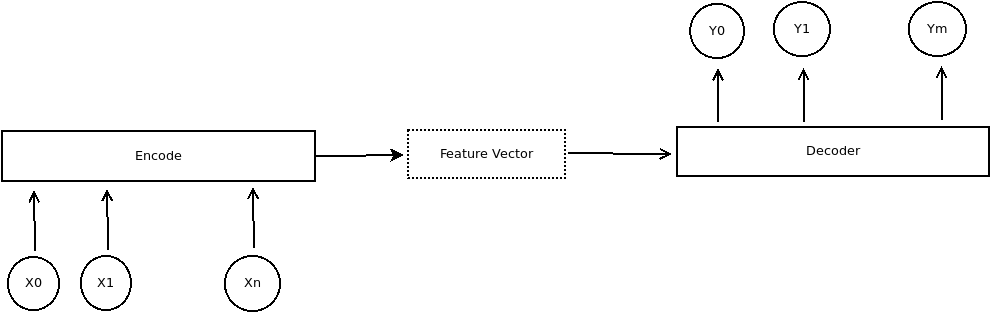
\includegraphics[scale=0.4]{Imgs/encoder_decoder.png}
			\caption{The basic scheme of the encoder-decoder model}
			\label{fig:encdec}
		\end{figure}
		
		\subsection{Encoder-Decoder Framework's Applications}
		The encoder-decoder framework is an architecture typically used to solve problems in which the model is supposed to generate a sequential output in response to a given input. The desired output is mostly in the form of a text describing the input.
		
		Some of the tasks in which the encoder-decoder model is used to solve the problem are as follows:
		\begin{enumerate}
			\item Machine Translation:\\
			"\textit{Machine translation}" (MT) is the task of generating a sentence in a destination language which has the same meaning as the given sentence from a source language. Two different approaches exists in machine translation. 
			
			The first approach, called "\textit{statistical machine translation}" (SMT), is characterized by the use of statistical machine learning techniques in order to automatically translate the sentence from the source language to the destination language. In less than two decades SMT has come to dominate academic machine translation research\cite{lopez2008statistical}. 
			
			The second approach is called "\textit{Neural Machine Translation}" (NMT). In this category, the encoder-decoder framework was first proposed by Cho et al. in 2014 \cite{cho2014learning}. In the Cho et al.'s model \cite{cho2014learning}, a neural network is used to extract features from the input sentence and another neural network is used to generate a sentence word by word from the destination language using the extracted feature vector. 
			
			In the neural structures used in NMT, a neural network is trained to map the input sequence (the input sentence as a sequence of words) to the output sequence. This kind of learning is known as "\textit{Sequence to Sequence Learning}".
			
			 Evaluations on the early models of NMT showed that although the generated translations are correct, the model faces extreme problems when translating long sentences\cite{cho2014properties}. The problem of modeling "\textit{long term dependencies}" is one of the most important challenges in the encoder-decoder models. We will drill into that and take a look at the proposed solutions, later in this chapter.
			
			\item Image/Video Captioning:\\
			Image captioning and video captioning are the problems of associating a textual description to a given image or video which holistically describes the objects and events presented in the input. A wide variety of approaches have been proposed to solve these problems, including probabilistic graphical models (PGMs) and neural encoder-decoder based models.
			
			Encoder-decoder based models for image captioning use a Convolutional Neural Network (CNN) as an encoder to extract a feature vector from the input image and pass it to a Recurrent Neural Network (RNN) as the decoder to generate the caption. The model architecture in this task is the same as that of machine translation except that the encoder uses a CNN to encode the image rather than an RNN.
			
			In video captioning, also called "\textit{video description generation}", a similar model based on the encoder-decoder architecture is employed to generate a caption for the input video. In video captioning models, the encoder typically consists of CNNs or combination of CNNs and RNNs to encode the input video and the decoder is the same as the decoder in machine translation and image captioning. 
			
			
			\item Textual/Visual Question Answering:\\
			Textual and visual question answering are the problems of generating an answer to a given question about an article and about an input image, respectively. Models proposed to solve these problems are supposed to generate a short or long answer, given a pair of an article and a question about it or an image and a question about it as the input. The base model architecture is then similar to that of machine translation except that the encoder is required to extract a feature vector for a pair of inputs. The decoder is the same as the decoder in machine translation and image/video captioning because it is supposed to generate a sentence describing the meaning of the feature vector generated by the encoder.
			
			\item Text Summarization:\\
			Proposed models for summarizing a text are supposed to generate a textual summary for the input text. The only constraint on the output is that it is required to describe the same meaning as the input text and its length should be shorter than that of the input. The base architecture of these models are the same as the architecture proposed in machine translation, except that the generated output here is from the same language as the input. 
			
		\end{enumerate}
	
	It can be easily seen that the baseline architecture proposed in machine translation is also used in other tasks with minor changes. In addition, the decoders of the models in different tasks are similar since most of them are used to generate a sentence word by word to describe the meaning of the input represented by the feature  vector. On the other side, a wide variety of encoders are used in order to extract appropriate feature vectors depending on the input types in different tasks. 
	
	\section{The encoder-decoder model for machine translation}
	Machine translation is the problem in which the encoder-decoder based models originated and proposed first. The Basic concepts of these models are shaped and presented in machine translation literature. So, in this section we will introduce the basic encoder-decoder structure proposed for machine translation by Cho et al. \cite{cho2014learning} to shed light on the model and its basics.
	
		\subsubsection{Formulation}
		Both the input and the output of machine translation models are sentences which can be formulated as a sequence of words. Let $X = \{x_0, x_1, \cdots, x_{L_{i}}\}$ denote the input sentence, where $x_i$ is the $i$th word in it assuming that the input sentence has $L_{i}$ words. Similarly, the output sentence could be formulated as $Y = \{y_0, y_1, \cdots, y_{L{o}}\}$ in which $y_i$ is the $i$th word in the output sentence assuming that it has $L_{o}$ words. Furthermore, all of $x_i$s and $y_i$s are one-hot vectors created from a dictionary of all words in the datasets.
		
		A one-hot vector is a vector whose components are all zero except for one of them. In order to create a one-hot vector for each word, first a dictionary\footnote{A dictionary is a list of unique words with unique indexes} of all possible words in the available datasets is created. Assuming $N$ words in the dictionary, an $N$-dimensional zero vector for each word is created and the component with the same index as the word in the dictionary is set to 1. Figure \ref{fig:onehot} demonstrates the one-hot vector for each word in a sample dictionary. Assuming the dictionary $D$ has 5 words "I", "cat", "dog", "have", "a" sequentially with the indices 0 to 4, one-hot vector for each word is displayed in the figure.
		
		\begin{figure}[H]
			\centering
			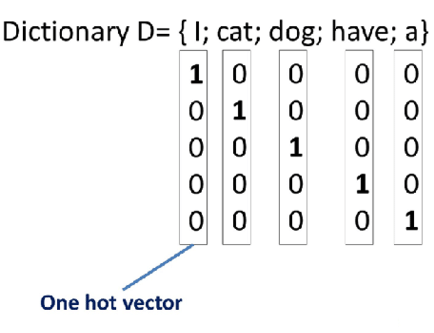
\includegraphics[scale=0.5]{Imgs/onehot.png}
			\caption{One-hot vector for each word in a sample dictionary. Sentences can also be modeled using \textit{Bag of Words} (BoW) technique in which the presence of a word in the sentence is considered without any information about the order of words.}
			\label{fig:onehot}
		\end{figure}
		
		The translation process is divided into the following two subprocesses:
		\begin{enumerate}
			\item Encoding phase: \\
			A recurrent neural network (RNN) is used to extract a feature vector from the input sentence from the source language. All of the words in the input sentence are converted to one-hot vectors and passed to the RNN in the order of their presence in the sentence. The RNN then updates its hidden state and output vectors according to each word. The iteration is stoped when the \textit{End of Sentence} (EOS) token is passed to the RNN. The EOS token is a token added manually to the end of input setences to determine the end point in the sentences. The hidden state of the RNN after the EOS token is then used as the feature vector of the input sentence. One-hot vectors of the words in the input sentence are created using the dictionary of words from the source language.
			\item Decoding phase: \\
			Another RNN is used to generate words of the output sentence in an appropriate order. The decoder RNN is designed to predict a probability distribution over all possible words in the dictionary of the source language words at each step. Then a word is selected with respect to the produced probability distribution as the next word in the sentence. The iteration is stopped when the EOS token is generated by the decoder or a predefined number of words are generated.
		\end{enumerate}
		
		The structure of the proposed model is show in figure \ref{fig:encdec1}. The context vector extracted by the encoder is denoted by $C$, which is the hidden state of the RNN encoder at the last step.
		\begin{figure}[H]
			\centering
			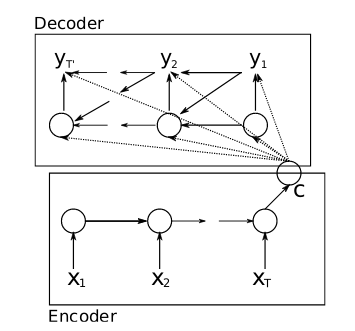
\includegraphics[scale=0.6]{Imgs/encdec1.png}
			\caption{An illustration of the first encoder-decoder based model proposed by Cho et al. \cite{cho2014learning}.}
			\label{fig:encdec1}
		\end{figure}
		
		\subsubsection{Encoders (feature extraction)}
		An RNN is used as the encoder in the model proposed by Cho et al.\cite{cho2014learning}. Let $h_e$ denote the hidden state of the encoder RNN. The hidden state of the encoder is updated at each time step $t$ according to equation \eqref{eq:hidden1} in which $h_e^t$ is the hidden state of the encoder at time step $t$, $f_{encoder}$ is a nonlinear activation function that can be as simple as an element wise logistic sigmoid function and as complex as a Long Short-Term Memory (LSTM), and $x_t$ is the one-hot vector of the $t$th word in the input sentence.
		
		\begin{equation}
			h_e^t = f_{encoder}(h_e^{t-1}, x_t)
			\label{eq:hidden1}
		\end{equation}
		
		Assuming that the input sentence has $L_i$ words, the encoder RNN should iterate on each word and update its hidden state vector at each step. The hidden state of the RNN after the $L_i$th word is then passed to the decoder as the context vector $C$. So, the context vector extracted by encoder can be computed as in equation \eqref{eq:context1}.
		\begin{equation}
			C = h_e^{L_i}
			\label{eq:context1}
		\end{equation}
		\subsubsection{Decoders (language modeling)}
		The decoder is supposed to generate the output sentence word by word in a way that the meaning of the sentence is the same as the meaning of the input sentence represented by the context vector $C$. From another point of view, the decoder can be seen as an RNN  that maximizes the likelihood of the translated sentence in the dataset for the input sentence and its generated context vector as expressed in \eqref{eq:obj1}, in which $\theta$ is the set of all trainable weights and parameters of the model.
		
		\begin{equation}
			Pr_\theta\{Y | X\}
			\label{eq:obj1}
		\end{equation}
		
		On the other hand, according to the encoder-decoder structure, the random variable $C$ directly depends on the random variable $X$, and the random varialbe $Y$ directly depends on the random variable $C$. Figure \ref{fig:BNI} displays the dependency graph between these 3 random variables.
		
		\begin{figure}[H]
			\centering
			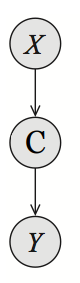
\includegraphics[scale=0.4]{Imgs/BNI.png}
			\caption{Directed Acyclic Graph of dependecies of random variables in the encoder-decoder model}
			\label{fig:BNI}
		\end{figure}
		
		 According to the dependencies displayed in figure \ref{fig:BNI}, it can be shown that $Y  \bigCI X | C$. Since $C$ is given we can replace the likelihood expressed in \eqref{eq:obj1} with the likelihood expressed in \eqref{eq:obj2}. Furthermore, assuming that each word in the sentence depends only on the meaning of the previous words in the sentence, the probability of a sentence can be replaced by the multiplication of the probabilities of its words given the previous ones.
		\begin{equation}
			Pr_\theta\{Y | C\} = \Pi_{t=0}^{L_o} Pr\{y_t| y_{t-1}, y_{t-2}, \cdots, y_0, C\}
			\label{eq:obj2}
		\end{equation}
		Consequently, the decoder is supposed to generate a probability distribution over each word at each step $t$ given its previously generated words and the context vector extracted by the encoder. The probability distribution can be formulated by the RNN according to equations \eqref{eq:obj3} and \eqref{eq:obj4}. Let $h_d^t$ be the hidden state of the decoder at time step $t$. Let $O^t$ be the decoder output at time step $t$ (an $L_o$ dimensional vector) which is generated by a nonlinear function $g$ applied on the decoder's hidden state and the context vector $C$. The decoder's hidden state is also generated by the nonlinear function $f_{decoder}$ applied on the previously generated word, hidden state of the decoder at previous time step and the context vector according to \eqref{eq:obj03}. With applying a softmax on the output, a vector with the same size is generated which sum of its components is equal to one and can be treated as the desired probability distribution.
		\begin{align}
			O^t &= g(h_d^t, y_{t-1}, C) 			\label{eq:obj3}\\
			Pr\{y_t| y_{t-1}, y_{t-2}, &\cdots, y_0, C\} = SoftMax(O^t)
			\label{eq:obj4}\\
			h_d^t = &f_{decoder}(h_d^{t-1}, y_{t-1}, C) \label{eq:obj03} 
		\end{align}
		At each time step, the probability distribution $Pr\{y_t| y_{t-1}, y_{t-2}, \cdots, y_0, C\}$ is generated by the decoder according to equation \eqref{eq:obj4} and the next word is selected with respect to this probability distribution over the words in the dictionary of the destination language.
		
		The two components of the proposed model can be jointly trained to minimize the negative conditional log likelihood expressed in \eqref{eq:loglikelihood1} in which $N$ is the number of samples in the dataset, $Y_n$ and $X_n$ are the $n$th output and input pair in the dataset, $\theta$ is the set of all trainable parameters, and $Loss$ is the loss function to be minimized.
		\begin{equation}
			Loss = -\frac{1}{N} \Sigma_{n=0}^N log Pr_\theta(Y_n | X_n)
			\label{eq:loglikelihood1}
		\end{equation}
		
%		\subsubsection{Results}
		
	\section{Encoder Structures}
	The baseline encoder-decoder architecture proposed by Cho et al. \cite{cho2014learning} in machine translation attracted the attention of many researchers in different fields. As explained before, almost all of the variants of the baseline architecture in different tasks share a similar decoder, but the structure of encoder varies based on the type of input. In this section, we will introduce the important structures of encoders to encode different input types.
		\subsection{Sentence as input}
		The simplest encoder for problems with sentences as inputs is an RNN. The first proposed encoder in machine translation is an LSTM which takes all words of the input sentence, processes them and returns its hidden state vector as the context vector. 
		
		Along with the RNNs, CNNs are employed to extract features from the source sentences in the encoding phase. As an instance, Gehring et al. proposed a convolutional encoder for machine translation in order to create better context vectors by taking nearby words into consideration using a CNN\cite{gehring2016convolutional}. In this encoder, a CNN with a kernel size of $k = 3$ is used to extract a combination of each three nearby words' meaning in the sentence to generate the context vector. 
		
		In addition, different RNN cells are used as blocks of the encoder for sentence inputs. LSTMs\cite{hochreiter1997long} are widely used because of their ability to cope with long term dependencies and remembering far history in the input sequence \cite{sutskever2014sequence}\cite{bahdanau2014neural}\cite{luong2015stanford}\cite{xu2015show}. GRU \cite{cho2014learning} is also used in different proposed models due to its good performance and the fact that it can be assumed as a light-weighted version of LSTM \cite{cho2014learning}\cite{mi2016coverage}\cite{he2016dual}\cite{tu2017context}.
		\subsection{Image as input}
		Encoder-Decoder based architectures form a majority of the proposed models to generate captions for images. In such models, the process of generating captions for the input image is divided into two steps. The first step is encoding in which a feature vector extracted from the image is returned as the context vector. The second step is decoding in which the generated context vector is passed to a decoder to generate sentences describing the context. 
		
		The best choice for encoders in such problems is the convolutional neural network. Almost all of the proposed models for image captioning based on the encoder-decoder framework use different types of CNNs as the encoders. Neural encoder-decoder based approaches to image captioning share the same structure for decoder, while in most of them the encoder consists of a single CNN. So, the extracted feature vector from the image can be expressed in \eqref{eq:imgCont} in which $X$ is the input image, $CNN(X)$ is the output of the CNN network, and $C$ is the context vector passed to the decoder.
		
		\begin{equation}
			C = CNN(X)
			\label{eq:imgCont}
		\end{equation} 
		
		A wide variety of CNNs are employed as encoders in the proposed models for image captioning. Since the pretrained versions of VGGNet \cite{simonyan2014very} and AlexNet \cite{krizhevsky2012imagenet} on the ImageNet dataset \cite{deng2009imagenet} extract good features from images for different tasks and are available online, they have been used as encoders in different proposed image captioning models \cite{karpathy2015deep} \cite{chen2017sca} \cite{pedersoli2017areas}. Furthermore, ResNet\cite{he2016deep} has been widely used because of its good performance as the encoder in such models \cite{lu2017knowing} \cite{rennie2017self} \cite{anderson2017bottom} \cite{yao2017boosting}. Google NIC Inception v3 \cite{szegedy2016rethinking} has also been used in proposed models because of its better image classification accuracy compared to ResNet \cite{zhang2017actor} \cite{ioffe2015batch} \cite{vinyals2015show} \cite{liu2017improved}. 
		
		Figure \ref{fig:imgCpt} illustrates the use of CNNs as the encoder in models based on the encoder-decoder framework for image captioning proposed by Vinyals et al. \cite{vinyals2015show}. A similar architecture is used to generate captions in other researches. As it is shown in the figure, the encoder part of the model consists of a CNN extracting feature vector from the input image. The extracted feature vector is then passed to the decoder to generate the appropriate caption. The decoder consists of an RNN which generates the probability of the next word according to \eqref{eq:obj2} at each step.
		
		\begin{figure}[H]
			\centering
			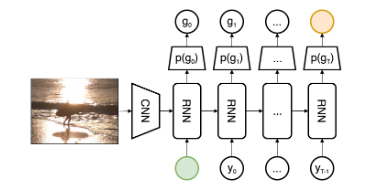
\includegraphics[scale=1]{Imgs/CNNImgCpt.png}
			\caption{Model architecture based on encoder-decoder framework for image captioning \cite{vinyals2015show}}
			\label{fig:imgCpt}
		\end{figure}
		
		\subsection{Video as input}
		Another sort of problems that the encoder-decoder models play an important role in solving them are those with videos as the input and describing text as the output, also called "\textit{Video Description Generation}" or "\textit{Video Captioning}". Since creating a good representation is critical to the overall performance of video captioning models, a wide variety of encoders are proposed to cope with different difficulties and challenges of such systems. This section presents some examples of encoders proposed to deal with the challenges of extracting motion details from the video.
		
		Assume an input video $V$ consists of $L_i$ frames. We can present the video as in equation \eqref{eq:vid1}, in which $v_i$ is a representation of the $i$th frame in the input video and $v_{L_i}$ is the end of video token (<EOV>). In fact, each $v_i$ is the feature vector extracted by a CNN on the $i$th frame in the input video.
		
		\begin{equation}
			V = \{v_0, v_1, \cdots, v_{L_i}\}
			\label{eq:vid1}
		\end{equation}
		
		Since in the baseline encoder-decode model, the encoder should return a "\textit{fixed length}" context vector extracted from the input an aggregation function is required to aggregate feature vectors from different frames in the video and pass it as the context vector to the decoder. 
		
		Different ideas have been employed to propose a good aggregation for video captioning. The first end-to-end encoder-decoder based approach in video description generation proposed by venugopalan et al. in 2014 \cite{venugopalan2014translating} used a mean pooling layer to create the fixed length context vector from the input video. In that model, first a CNN is applied to each frame of the input video. Then a mean pooling layer is applied to create an average feature vector over the set of feature vectors extracted from each frame. The average feature vector is then passed to the decoder to generate the sentence. A stacked RNN structure is used as the decoder.
		
		\begin{figure}[H]
			\centering
			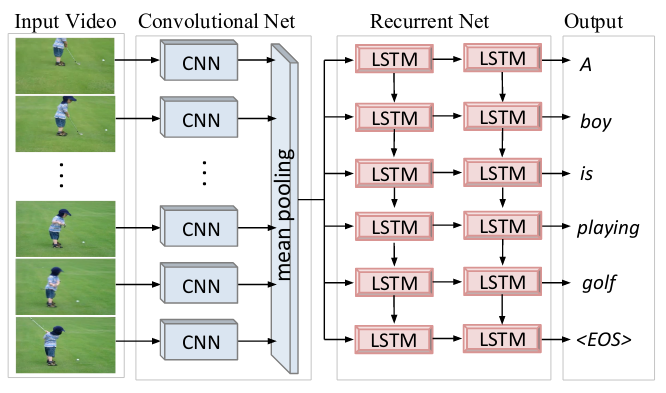
\includegraphics[scale=0.5]{Imgs/vid1.png}
			\caption{An illustration of the first encoder-decoder based model for video description generation proposed by venugopalan et al. in 2015 \cite{venugopalan2014translating}}
			\label{fig:vid1}
		\end{figure}
	
		Different CNNs have been used to extract feature vectors from frames of the input video. For instance, Yao et al. \cite{yao2017boosting} used Inception V4 \cite{szegedy2017inception} for feature extraction from video frames.
	
		Extracting good features from the input video is a challenging task that can highly affect the performance of the proposed model. The extracted context vector from the input video should well express the detailed motions in the video. In order to create an encoder which is able to extract fine motion features from the video, Yao et al. \cite{yao2015describing} proposed a 3D-CNN as the encoder. The structure of this 3D-CNN is illustrated in figure \ref{fig:3dcnn}.
		
		\begin{figure}[H]
			\centering
			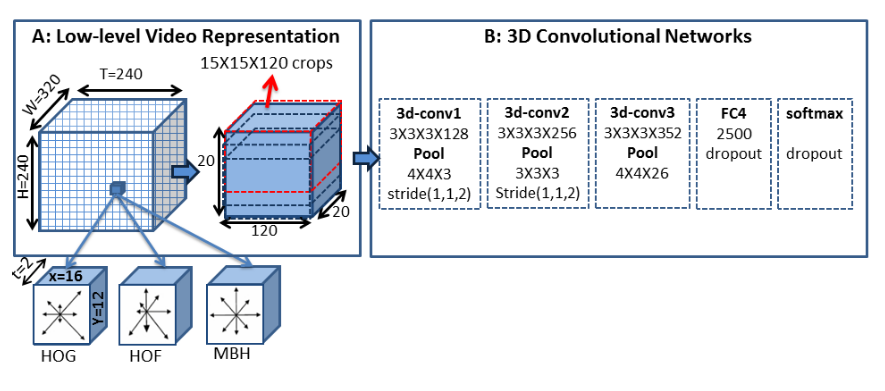
\includegraphics[scale=0.5]{Imgs/3DCNN.png}
			\caption{The structure of 3D-CNN proposed by Yao et al. in 2015 \cite{yao2015describing}}
			\label{fig:3dcnn}
		\end{figure}
	
		Actually, the proposed 3D-CNN models the spatio-temporal dependencies in the input video. The 3D-CNN is used to build a higher-level representation that preserves the local motion information from short frame sequences in the input video. This is accomplished by first dividing the input video clip into a 3D spatio-temporal grid of $16 * 12 * 2$ (width * height * timesteps) cuboids. Each cuboid is represented by concatenating the histogram of oriented gradients (HoG), histogram of oriented flow (HoF) and motion boundary histogram(HoG, HoF, MbH) with 33 bins. This transformation ensures that local temporal structures and motion features are well extracted. The generated 3D descriptor then is passed to 3 convolutional layers each followed by a max-pooling layer and one fully connected layer followed by a softmax layer as demonstrated in the figure \ref{fig:3dcnn}. The output of the 3D-CNN is then passed to the decoder to generate an appropriate caption.
		
		The 3D-CNN proposed by Yao et al. \cite{yao2015describing} is also used along side the typical 2D-CNN in other works. Pan et al. \cite{pan2016jointly} proposed a novel encoder-decoder architecture for video description generation and used the 3D-CNN and the typical 2D-CNN and applied a mean pooling layer to the set of extracted features by each of the CNNs and concatenated the output to generate the context vector of the video. Figure \ref{fig:3dcnn2} illustrates the encoder part of this model.
		
		\begin{figure}[H]
			\centering
			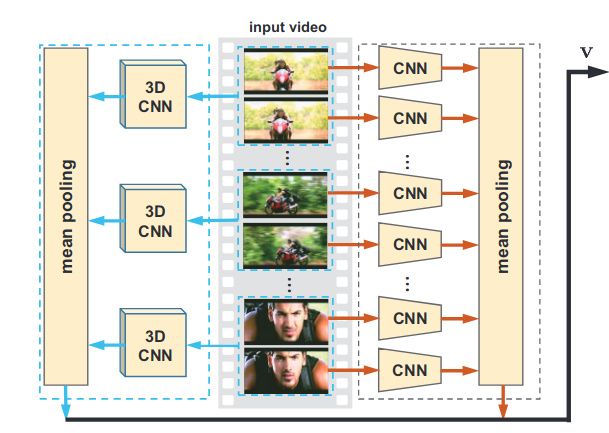
\includegraphics[scale=0.5]{Imgs/3DCNN2.png}
			\caption{An illustration of the encoder part of the proposed model by Pan et al. \cite{pan2016jointly}}
			\label{fig:3dcnn2}
		\end{figure}

		Another approach to video captioning includes those methods focusing on "\textit{Dense Video Captioning}". Despite the models that generate a single sentence as the description of the input video, dense video captioning models first detect and localize the existing events in the input video and then generate a description sentence for each of the detected events. 
		
		Encoders for dense video captioning are supposed to first detect all of the existing events in the input video. Then for each of the events a quadruple <$t_{start}$, $t_{end}$, $score$, $h$> should be extracted. $t_{start}$ and $t_{end}$ are the starting and ending frame numbers of the specified event. $score$ is the confidence score of the encoder for each of the events. If the $score$ of an event is greater than a threshold, it is reported as an event and its quadruple is passed to the decoder for sentence generation; otherwise, it is ignored. Finally $h$ is the feature vector extracted from the range of frames between $t_{start}$ and $t_{end}$ which is used by the decoder as the context vector of the event to generate a sentence for te event \cite{li2018jointly}. 
		
		The task of dense video captioning was proposed by Krishna et al. \cite{krishna2017dense} first in 2017. The proposed encoder by Krishna et al. \cite{krishna2017dense} for dense video captioning is able to identify events of the input video within a single pass while the proposed decoder simultaneously generates captions for each event detected and passed by the encoder.
		
		Figure \ref{fig:dense1} illustrates the structure of encoder proposed by Krishna et al. \cite{krishna2017dense} for dense video captioning. The proposed encoder is able to extract all events in the input video using a deep action proposal(DAP) module proposed by \cite{escorcia2016daps}. To do this, a 3D-CNN is applied to the input video frames to extract video features. These video features are passed to the DAP module. This module consists of different LSTMs that are applied to the video features sequence in different resolutions and are trained to detect starting and ending points of events. The confidence score of each event is also computed by DAP. The proposed event proposals are then sorted with respect to their ending points and passed sequentially to the decoder. The feature vector of each event is also the hidden state of the corresponding RNN in the DAP. The decoder then generates a sentence for each event using its feature vector as the encoder output.
		
		\begin{figure}[H]
			\centering
			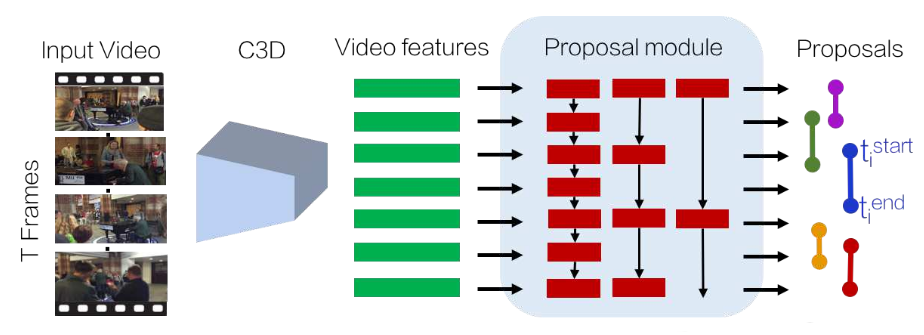
\includegraphics[scale=0.4]{Imgs/dense1.png}
			\caption{An illustration of the first proposed encoder model for dense video captioning by Krishna et al. \cite{krishna2017dense}}
			\label{fig:dense1}
		\end{figure}
	
		Li et al. \cite{li2018jointly} proposed a novel end-to-end encoder-decoder based approach for dense video captioning which unified the temporal localization of event proposals and sentence generation\cite{li2018jointly}. Figure \ref{fig:dense2} illustrates the structure of this model. \cite{li2018jointly}. Here, instead of using an extra DAP module, a 12 layer convolutional structure is designed to extract features for action proposal over the output of the 3D-CNN. The first 3 layers of the convolutional structure (500D layer and base layers in figure \ref{fig:dense2}) are designed to introduce nonlinearities and decrease the input dimension. The next 9 layers, which are called "Anchor layers", extract features from different resolutions to be used for event prediction. The "Prediction Layer" consists of three parallel fully connected layers to first regress temporal coordinates ($t_{start}$ and $t_{end}$) of each event, then compute the descriptiveness of the event ($score$) and finally classify the event vs background. The prediction layer is applied to the output of all anchor layers to enable the model to detect events from different resolutions. The extracted proposals are then passed to the proposal ranking module which ranks event proposals with respect to their ending time. Finally the events are passed to the decoder for sentence generation sequentially.
		
		\begin{figure}[H]
			\centering
			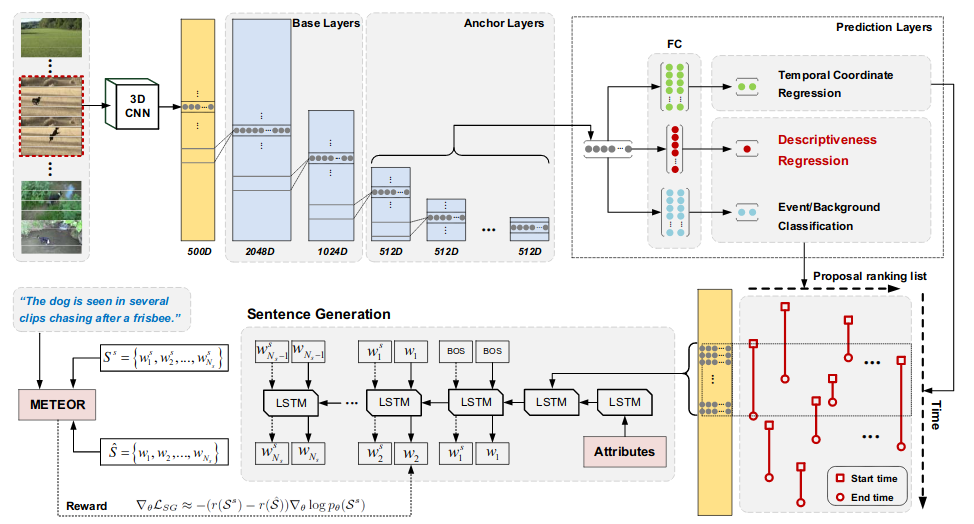
\includegraphics[scale=0.5]{Imgs/dense2.png}
			\caption{An illustration of the encoder-decoder structure proposed by Li et al. for dense video captioning \cite{li2018jointly}}
			\label{fig:dense2}
		\end{figure}
	
		A wide variety of models are proposed to cope with the difficulties of the encoding phase in dense video captioning. Shen et al. \cite{shen2017weakly} proposed a new CNN called "\textit{Lexical FCN}" which is trained in a weakly supervised manner to detect events based on the captions in the dataset. Duan et al. also proposed a novel approach for dense video captioning based on the similar assumption "each caption describes one temporal segment, and each temporal segment has one caption"\cite{duan2018weakly}. Xu et al. proposed an end-to-end encoder-decoder based model for dense video captioning which detects and describes events in the input video jointly and is applicable to dense video captioning on video streams. Zhou et al. also proposed an end-to-end approach with a masking network to localize and describe events jointly\cite{zhou2018end}. Wang et al. proposed a novel architecture to take both past and future frames into account while localizing the events in the input video \cite{wang2018bidirectional} using bidirectional models. 
	
	\section{Decoder Structures}
	In the encoder-decoder based models, decoders generate a sequential output for the given input. The output is mostly in the form of a descriptive text. Therefore, the main structures of the decoders are similar in different tasks. This section, introduces different techniques proposed to make better decoders with better generated captions. 
		\subsection{Long term dependencies}
		One of the basic problems with RNNs is the problem of "\textit{long term dependencies}". Indeed, in these networks when the length of the input or the length of the desired output is too large, the gradients should propagate over many stages. When the gradient is propagated over a large number of stages, they tend to either vanish or explode.
		
		 In addition, the gradients in each backpropagation step are multiplied by small coefficients or small learning rates. Thus, the gradient in the early stages will be close to zero and might make no changes in the weights of the early stage layers\cite{goodfellow2016deep}. 
		
		In this section we will discuss the approaches proposed to cope with the long term dependencies challenge in the decoders.
		
		\subsection{LSTMs}
		LSTMs have achieved strong results on a variety of sequence modeling tasks thanks to their superior ability to preserve sequence information over time. The combination of the "\textit{memory cell}" and the "\textit{forget gate}" in the structure of LSTM improves the ability of LSTM to model sequence information by training to forget unnecessary information (using forget gate) and keep necessary information in the memory cell. Cho et al. \cite{cho2014learning}, Bahdanau et al.\cite{bahdanau2014neural}, Luong et al. \cite{luong2015effective}, Wu et al. \cite{wu2016google}, Johnson et al. \cite{johnson2017google} and Luong et al. \cite{luong2014addressing} used LSTMs as both the encoder and decoder part of their models proposed for machine translation because of the LSTM's power to remember far away points.
		\subsection{Stacked RNNs}
		As mentioned earlier, multi-staged decoders are hard to train due to the vanishing gradient problem. Thus most of the proposed encoder-decoder based models use a single layer RNN as the decoder which results in difficulties to generate rich fine-grained sentences. Stacking multiple RNNs on top of each other is another way to enable decoders to generate sentences describing more details of the input image.
		
		Donahue et al. \cite{donahue2015long} proposed an encoder-decoder based approach to image captioning which uses a stacked structure of LSTMs as the decoder in order to describe more details of the input image. In this proposed method an LSTM is used on top of another one in the way that the first layer LSTM takes image features and the previously generated word embedding along with its previous hidden state vector as the input and generates a coarse low-level representation of the output sentence. In the next step the hidden state of the low level LSTM is passed to the next LSTM as input along with its previous hidden state to generate fine high-level representation of the output. A softmax layer is then applied to the generated high-level representation of the output to generate the probability distribution of the next word in the sentence. Gu et al. \cite{gu2018stack} also used en encoder-decoder based model with a two-layer stacked LSTM as decoder in order to enable the proposed model to generate better descriptions.
		
		The idea of employing a stacked structure of RNNs as the decoder is also used in models proposed for video description generation. Venugopalan et al. \cite{venugopalan2014translating} proposed the first decoder in neural encoder-decoder based approaches for video description generation with a simple stacked structure. Figure \ref{fig:stacked} demonstrates the architecture of a sample stacked decoder. Blocks tagged with "C" display the input at each step. The red line illustrates the shortest path from the first step to the output in the model. Since the length of the shortest path from the first step to the output correlates with the testing and the training time of the model, decreasing this length decreases the testing and the training time of the model. 
		
		
		\begin{figure}[H]
	\centering
	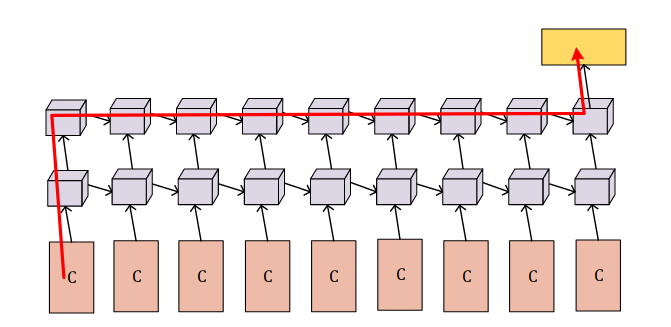
\includegraphics[scale=0.5]{Imgs/stacked.png}
	\caption{Stacked structure of RNNs \cite{pan2016hierarchical}}
	\label{fig:stacked}
\end{figure}

		Along with the methods using stacked RNNs as decoders, a category of models are proposed which follow a hierarchical fashion to arrange RNNs in decoders in order to enable the models to generate fine-grained output sequences. 
		
		In addition, hierarchical RNN structures are also used to enable encoders in the problems with a sequential input to exploit and encode more detailed information from the input. Pan et al. \cite{pan2016hierarchical} proposed an encoder-decoder based model for video description generation with a hierarchical encoder structure. In their model, two layers of different LSTMs are used. The first layer LSTM is applied to all sequence steps in order to exploit low-level features and the second layer LSTM is applied on the output of equally sized subsets of the input sequence steps to exploit the high-level features. Figure \ref{fig:hrne} demonstrates this architecture. The illustrated red line, shows the shortest path from the first step to the output. Comparing structures displayed in figures \ref{fig:stacked} and \ref{fig:hrne} shows that the shortest path from the first step to the output in hierarchical models is much smaller than that of stacked models. Therefore, the efficiency of the hierarchical model is much higher than that of the stacked model.
				\begin{figure}[H]
			\centering
			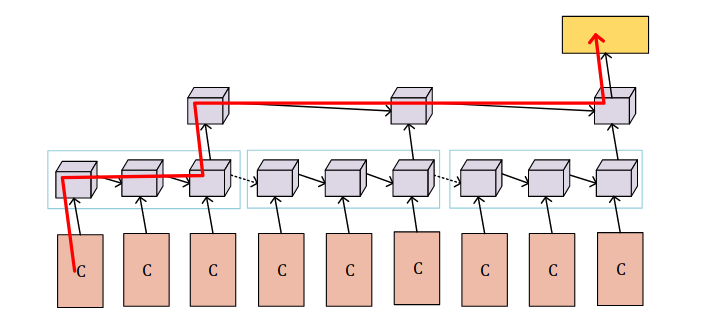
\includegraphics[scale=0.5]{Imgs/hrne.png}
			\caption{Hierarchical structure of RNNs \cite{pan2016hierarchical}}
			\label{fig:hrne}
		\end{figure}
		More complex hierarchical structures are also proposed in the literature for different intents. Yu et al.\cite{yu2016video} proposed a model with a hierarchical structure to generate a set of sentences arranged in a single paragraph as a description for the input video. The first layer in this model is a simple decoder to generate single sentences and the second layer is a "\textit{paragraph controller}". The paragraph controller is another RNN which generates a feature vector given the last hidden state of the first layer RNN denoting the meaning of the next sentence to be generated. The first layer RNN then takes the feature vector generated by the second layer and concatenates it with other inputs to control the meaning of the next sentence.
				
		\subsubsection{Vanishing gradients in stacked decoders}
		Even though increasing the depth of the stacked decoder structure adds more nonlinearities to the model and empowers it to generate fine-grained sentences, the number of layers in the stacked structures is strictly restricted. Most of stacked decoder structures use at most 2-layers of RNNs on top of each other \cite{donahue2015long} \cite{pan2016hierarchical} \cite{yu2016video}. 
		
		Indeed, the most important issue restricting the number of layers in stacked structures is the problem of vanishing gradients in deeper decoders. The backpropagated gradients vanish as a result of two facts. First, the gradients in such architectures are multiplied by small multipliers and small learning rates at each stage. Second, since the loss function of the proposed decoders is based on the likelihood of the next word, decoders are supposed to predict a probability distribution over all the words in the dictionary. It means the decoder's output size is equal to the size of word dictionary. Furthermore, the sum of all components in the output layer is supposed to be equal to 1, which means the gradients computed at the last layer are numerically small. Summing up, the gradients vanish in stacked decoders since the computed gradients at the last layer are small and they are multiplied by small multipliers at each step.
		
		Asadi et al. \cite{Asadi2019stacked} proposed a novel approach to train the stacked decoders in a way that the gradients of the last layer are large enough to make significant changes in weights of the first layers. The main idea is to use a word-embedding vector instead of one-hot vector representation as the decoder desired output. As a result, the optimization problem changes from predicting the conditional probability distribution of the next word to a word-embedding regression and the \textit{Softmax} layer at the end of the decoder is removed. In this way, the limitations of the value of the computed gradients at the last step are resolved. In addition, the loss function of the decoder is changed from the cross-entropy to MSE of the word embedding of the next word.
		
		\subsection{Reinforcement learning}
		One of the problems of training the decoders using the loglikelihood model is that the performance of the model is highly different on the training and testing sets. This occurs since the optimization function for training is different from the evaluation metrics used in testing. Recently, reinforcement learning has been used to decrease the gap between training and testing performance of the proposed models. In other words, the main problem with loglikelihood objective is that it does not reflect the task reward function as measured by the BLEU score in translation. 
		
		Wu et al. \cite{wu2016google} proposed the first decoder trained by reinforcement learning for machine translation. After that, other researchers used reinforcement learning to train decoders in other tasks. Wang et al. \cite{wang2018video} proposed the first decoder trained with reinforcement learning taking CIDEr\cite{vedantam2015cider} score as reward in video captioning. Li et al. \cite{li2018jointly} also trained a decoder in a reinforcement learning fashion using the METEOR \cite{banerjee2005meteor} score as reward to generate caption for the input videos. 
		
		Figure \ref{fig:reinf1} illustrates the structure of the model proposed by Wang et al.\cite{wang2018video}. The decoder in this work consists of three different modules, namely a manager, a worker, and an internal critic. These three modules are trained using a reinforcement learning method. The manager operates at a lower temporal resolution and emits a goal when needed for the worker, and the worker generates a word for each time step by following the goal proposed by the manager. The internal critic determines if the worker has accomplished the goal and sends a binary segment signal to the manager to help it update goals. 
		
		\begin{figure}[H]
			\centering
			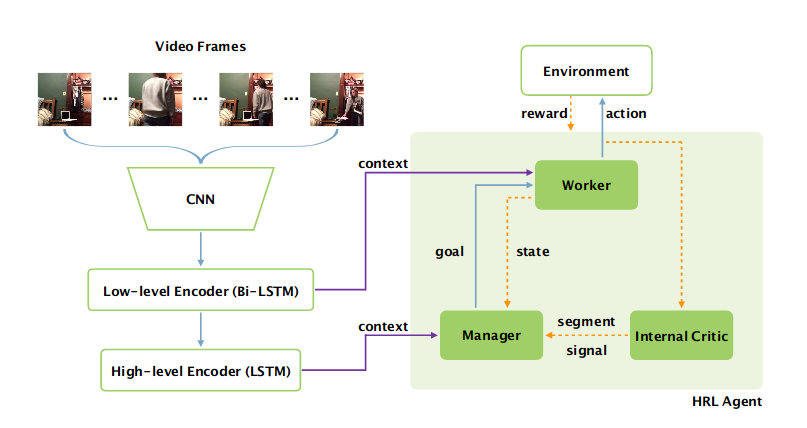
\includegraphics[scale=0.5]{Imgs/reinf1.png}
			\caption{An illustration of the encoder-decoder based model proposed by Wang et al. \cite{wang2018video}. The proposed decoder is trained using reinforcement learning.}
			\label{fig:reinf1}
		\end{figure}
	
		Figure \ref{fig:reinf2} illustrates the unrolled decoder proposed by Wang et al. The manager takes the context vector $c_t^M$ at time step $t$ and the feature vector of sentence generated at previous time step $h_{t-1}^W$ as input. An LSTM is used to model extracted goal sequences. The LSTM takes the input and updates it hidden state $h_t^M$. The hidden state of the LSTM is then used to generate next goal using the nonlinear function $u_M()$ according to \eqref{eq:reinf2}.
		
		\begin{align}
			h_t^M = LST&M^M(h_{t-1}^M, [c_t^M, h_{t-1}^W]) \label{eq:reinf1} \\
			g_t &= u_M(h_t^M) \label{eq:reinf2}
		\end{align}
		
		$LSTM^M$ denotes the LSTM function used in manager, $u_m$ is the function projecting hidden states to the semantic goal, $h_{t-1}^M$ is the hidden state of the manager LSTM at previous time step, and $g_t$ is the vector of semantic goal generated at time step $t$.
		
		\begin{figure}[H]
		\centering
		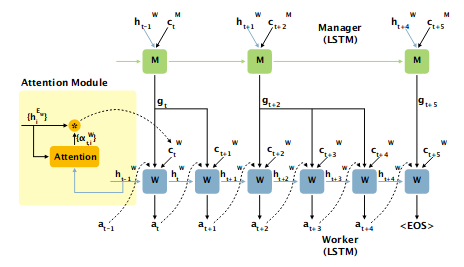
\includegraphics[scale=0.8]{Imgs/reinf2.png}
		\caption{An illustration of the unrolled decoder proposed by Wang et al. \cite{wang2018video}.}
		\label{fig:reinf2}
	\end{figure}
	
		The worker then receives the generated goal $g_t$, takes the concatenation of $[c_t^W, g_t, \alpha_{t-1}]$ as the input, and outputs the probabilities $\pi_t$ over all actions $\alpha_t \in V$, where each action is a generated word according to equations \eqref{eq:reinf3} to \eqref{eq:reinf5}.
		
		\begin{align}
			h_t^W = LSTM^W(h_{t-1}^W, [c_t^W, g_t, \alpha_{t-1}]) \label{eq:reinf3} \\
			x_t = u_W(h_t^W) \label{eq:reinf4} \\
			\pi_t = SoftMax(x_t) \label{eq:reinf5} 
		\end{align}
		
		The internal critic is used to provide a good coordination between the manager and the worker. Internal critic is indeed a classifier to determine when the worker is done with generating an appropriate phrase for a given goal. When the worker is done, internal critic sends an activation signal to manager to generate a new goal. Let $z_t$ be the binary signal of the internal critic, the probability $Pr(z_t)$ is computed according to equations \eqref{eq:reinf6} and \eqref{eq:reinf7}.
		
		\begin{align}
			h_t^I = LSTM^I(h_{t-1}^I, \alpha_t]) \label{eq:reinf6} \\
			Pr(z_t) = sigmoid(W_zh_t^I + b_z) \label{eq:reinf7} \\
		\end{align}
		
		The objective of the worker is to maximize the discounted return \eqref{eq:drtn} in which $\theta_W$ is the set of trainable parameters of the worker, $\gamma$ is the discount rate, and $r_{t+k}$ is the reward at step $t+k$. Therefore, the loss function of the decoder can be written as \eqref{eq:reinf8}.
		
		\begin{align}
			R_t = \Sigma_{k=0}^\infty \gamma^k r_{t+k} \label{eq:drtn} \\
			L(\theta_W) = -E_{\alpha_t \sim \pi_{\theta_W}}[R(\alpha_t)] \label{eq:reinf8}		
		\end{align}
		The gradient of the non-differentiable, reward-based loss function can be derived as:
		
		\begin{equation}
			\nabla_{\theta_W} L(\theta_W) = - E_{\alpha_t \sim \pi_{\theta_W}} [R(\alpha_t \nabla_{\theta_W} log \pi_{\theta_W}(\alpha_t))]
		\end{equation}
		
		Typically the expectation of the loss function if estimated with a single sample, so the expectation term can be omitted. In addition, the reward can be subtracted with a baseline $b_t^W$ in order to generalize the policy gradient.
		
		\begin{equation}
			\nabla_{\theta_W} L(\theta_W) \approx -(R(\alpha_t - b_t^W) \nabla_{\theta_W} log \pi_{\theta_W} (\alpha_t)
		\end{equation}
		
		The manager is supposed to be trained in a way that it can compute goals to generate sentences with better BLEU scores and the action of the decoder is produced by the worker. So, the worker is assumed to be fully trained and used as a black box when training the manager. More specifically, the manager outputs a goal $g_t$ at step $t$ and the worker then runs $c$ steps to generate the expected segment $e_{t, c} = \alpha_t \alpha_{t+1} \alpha_{t+2} \cdots \alpha_{t+c}$ using the goal. Then the environment responds with a new state $s_{t+c}$ and reward $r(e_t, c)$. Following a similar math, final gradients to train manager can be derived as in \eqref{eq:nabla}.
		
		\begin{equation}
			\nabla_{\theta_M} L(\theta_M) = -(R(e_t, c) - b_t^M) [\Sigma_{i=t}^{t+c-1} \nabla_{g_t} log \pi(\alpha_i)] \nabla_{\theta_m} \mu_{\theta_M} (s_t)
			\label{eq:nabla}
		\end{equation}
		
		In which $\mu_{\theta_M} (s_t)$ is a noisy version of the generated goal and is used in order to empower exploration in the training of the model. Furthermore, rewards are defined as \eqref{eq:reinf9} and \eqref{eq:reinf10}.
		
		\begin{align}
			R(a_t) = \Sigma_{k=0}^\infty \gamma^k [CIDEr(sent + \alpha_{t+k}) - CIDEr(sent)] \label{eq:reinf9} \\
			R(e_t) = \Sigma_{n=0}^\infty \gamma^n [CIDEr(sent + e_{t+n}) - CIDEr(sent)] \label{eq:reinf10} 
		\end{align}
		
		Other metrics such as BLEU score can be used instead of CIDEr \cite{papineni2002bleu}.
		
	\section{Attention Mechanism}
		Models based on the encoder-decoder framework encode input to a "\textit{fixed length vector}". The decoder in these models generates the output based on the information represented in the fixed length encoder output. Each element of the output may be more strongly related to a specific part of the input. In these cases, more detailed information about that specific part of the input is required, and the extra information from the other parts of the input could deceive the model. 
		
		Attention mechanism, first introduced by Bahdanau et al. \cite{bahdanau2014neural} in machine translation, is a mechanism that allows the encoder-decoder models to pay more attention to a specific part of the input, while generating the output at each step. Furthermore, the mechanism enables decoders to cope with the long term dependencies and generate more fine-detailed sentences and outputs.
		
		In this section, first the basic idea of the attention mechanism proposed in machine translation is described. Then, the use of this mechanism in some encoder-decoder architectures proposed various applications is discussed.
		
		\subsection{Basic Mechanism}
		Bahdanau et al. \cite{bahdanau2014neural} proposed the first encoder-decoder based model equipped with the attention mechanism in order to produce better translations. The encoder and the decoder parts of the proposed model are changed. The encoder is modified to generate a sequence of feature vectors called "\textit{annotation vectors}" and an extra layer called "\textit{attention layer}" is added in between the encoder and the decoder. The attention layer, receives the annotation vectors generated by the encoder and creates a fixed length context vector at each step and passes it to the decoder in order to generate the probability of the next word in the sentence.
		
		Based on these changes, the target probability distribution of the decoder can be expressed as in \eqref{eq:attn1}. It denotes the probability of the next word $y_t$ at time step $t$, given all of the previously generated words and the context vector generated to predict the $t$th word. The decoder computes this probability at each step.
		
		\begin{equation}
			Pr(y_t | y_{t-1}, \cdots, y_0 , C_t)
			\label{eq:attn1}
		\end{equation}
		\\
		Let $L = \{l_0, l_1, \cdots, l_{N_i}\}$ be the set of generated annotation vectors by the encoder, and $N_i$ be the number of generated annotations, the context vector $C_t$ is then computed at each step using the equation \eqref{eq:attn2}. The coefficients $\alpha_k$ in \eqref{eq:attn2} are called the "\textit{attention weights}".
		
		\begin{equation}
			C_t = \Sigma_{k=0}^{N_i} \alpha_k^t l_k
			\label{eq:attn2}
		\end{equation}
		\\
		The keypoint in generating the context vector at each step using the attention mechanism is to compute the attention weights at each step. Researchers have proposed different ways to compute the attention weights. One of the most used attention mechanisms which is called "\textit{Soft Attention}", is proposed by Xu et al. \cite{xu2015show}. The attention weights in soft attention are computed using equations \eqref{eq:attn3} and \eqref{eq:attn4}.
		
		\begin{align}
			\alpha_k^t = \frac{exp(e_k^t)}{\Sigma_{j=0}^{N_i} exp(e_j^t)} \label{eq:attn3}\\
			e_k^t = f(h_{t-1}, l_j) \label{eq:attn4}
		\end{align}
		
		Equation \eqref{eq:attn4} is an alignment model which scores how well the output at step $t$ depends on the input section related to the annotation vector $l_j$. The function $f$ in \eqref{eq:attn4} measures the alignment between the output and the input. A simple candidate for implementing function $f$ is an MLP which can be modeled as:
		
		\begin{equation}
			f(h_{t-1}, l_j) = W_2 tanh(W_h h_{t-1} + W_l l_{j} + b_1) + b_2
		\end{equation}
		
		In which $W_2$, $W_h$, and $W_l$ are weight matrices and $b_1$ and $b_2$ are biases. All of these parameters can be trained jointly with other trainable model parameters.
		
		Another version of the attention mechanism, called "\textit{Hard Attention}", is also introduced by Xu et al. \cite{xu2015show} in which at each step one of the attention weights is equal to 1 and the rest are equal to zero. 
		
		\subsection{Extensions}
		Attention mechanism is also used in other tasks. You et al. \cite{you2016image} proposed a semantic attention in image captioning. Lu et al. \cite{lu2017knowing} also proposed an adaptive version of the attention mechanism in image captioning. Gao et al. proposed an encoder-decoder based model using the attention mechanism and introduced a novel approach to train the attention weights to decrease the semantic gap of the generated caption. Wu et al. \cite{wu2018hierarchical} also proposed a novel encoder-decoder based model for video captioning which is able to select from different information sources like motion, temporal, audio and semantic features of the input video to generate caption describing the input video.

		\section{Conclusion}
		
	\bibliography{ref}
	\bibliographystyle{ieeetr}
\end{document}